\documentclass{standalone}
\usepackage[dvipsnames]{xcolor}
\usepackage{tikz}

\usepackage[sfdefault,black]{merriweather} %% Option 'black' gives heavier bold face 
\usepackage[T1]{fontenc}

\begin{document}
	
	\begin{tikzpicture}[inner sep=0pt,outer sep=0pt]
		
		\pgfmathsetmacro{\a}{0.03};
		\pgfmathsetmacro{\R}{0.25};
	
%		\begin{scope}[local bounding box=scope1]
%			
%		\node at (0,0) {\includegraphics[width=2.5cm]{sucrose.pdf}};
%				
%		\end{scope}
%	
%		\begin{scope}[shift={($(scope1.center)+(0.0cm,0.0cm)$)}]
%			
%		\node[font=\small,color=Venus] at (0,0) {s\textsc{ub}\emph{\color{IndianRed}hkl}};
%	
%		\end{scope}
		
		\begin{scope}[local bounding box=scope1]
	
		\node at (0,0) {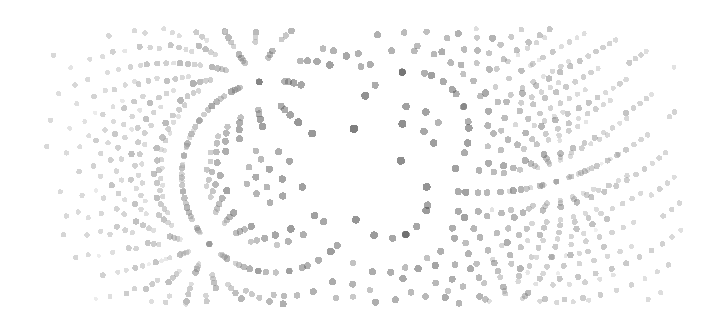
\includegraphics[width=2.2cm]{5VNQ.pdf}};
		\node[font=\LARGE,color=black,opacity=0.666] at (0,0) {s\textsc{ub}\emph{\color{RubineRed}hkl}};	
		\end{scope}
				
%		\begin{scope}[shift={($(scope1.east)+(1cm,0cm)$)}]
%			
%		\node[font=\LARGE,color=Venus] at (0,0) {s\textsc{ub}\emph{\color{CarnationPink}hkl}};
%
%		\end{scope}
%		
	\end{tikzpicture}
	
\end{document}